\documentclass[10pt]{article}
\usepackage{commands}


\begin{document}
%Course webpage: https://phas.ubc.ca/~seme/516/
\begin{tcolorbox}
  \begin{center}
  \begin{Large}
    \textbf{PHYS 516 (Statical Mechanics) Notes} \\
    \vspace{5pt}
  \end{Large}
  \begin{large}
        Rio Weil \\
\vspace{5pt}
    \emph{This document was typeset on \today}
  \end{large}
  \end{center}
\end{tcolorbox}
% Email: gordonws@phas.ubc.ca
% Office: Henn 344
% Webpage: https://phas.ubc.ca/~seme/516/


\begin{center}
  \textbf{Introduction:}

  This is a set of lecture notes taken from UBC's PHYS 516 (Graduate Statistical Mechanics) course, taught by Dr. Gordon Semenoff. The course covers fundamentals of statistical mechanics, phase transitions and critical exponents, $D = 1,2,3$ Ising models, mean field theory, quantum field theory, universality, renormalization, and elementary conformal field theory. If any errors are found in the notes, feel free to email me at \href{mailto:ryoheiweil@phas.ubc.ca}{ryoheiweil@phas.ubc.ca}.
\end{center}
\addtocontents{toc}{\protect\hypertarget{toc}{}}
\tableofcontents

\newpage
\section{Introduction, Statistical Mechanics Review}

\subsection{Overview}
This course centers around critical phenomena and phase transitions (primarily in magnetic systems/the Ising model) - PHYS 403 is a more comprehensive overview of the field, this is more specialized. We will discuss models that are analytically solvable (or almost), some renormalization group methods, some conformal field theory and the conformal bootstrap method.

We will begin with a review of some basic statistical mechanics. In a nutshell, statistical mechanics is the application of probability theory to a physical system - typically, with a large number of degrees of freedom as this is the limit where the application is useful. Perhaps saying probability theory is a bit reaching, though - the probability involved is pretty minimal (lots of counting, not a ton of measure theory). It is worth noting that (much like other fields of physics) there are very few systems that are analytically solvable; most systems require the application of approximate techniques.

\subsection{Canonical Ensemble}
There are various places to begin this discussion; let's start by discussing the canonical ensemble. Let us consider a physical system, which has an array of possible states. Let us assume that it is characterized by energies $E_a$, and the energy can take up one out of a list of possible values $E_1, E_2, E_3, \ldots$. Given the conservation of energy for a closed system, this is a reasonable way to characterize a state (and given one of our goals of doing thermodynamics with our system, this is a useful quantity). Let us not say too much more about the system - other than perhaps the fact that the energy has a lower bound (but not necessarily an upper bound), and that the energies are ordered. Further, for now let us assume that the energies are discrete - this is of course not true in general (there exist systems for which energy is a continuum, and there we will have to use some kind of binning procedure), but let us assume this simplification for now.

So, how do we make the canonical ensemble? We take $\N$ copies of the system, with various energies, so that $\mathcal{E} = \sum_{i=1}^{\N} E_i$ is the total energy. The $\N$ copies of the system are weakly coupled to each other. This means that energy can flow between the systems, but also that (since the coupling is weak) when we calculate the total energy we can neglect the interaction energies between the systems. In other ensembles, other things that are not the energy can be exchanged (e.g. particles in the grand canonical ensemble).

\begin{figure}[htbp]
    \centering
    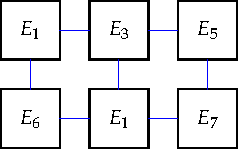
\includegraphics[]{Images/fig-canonicalensemble.pdf}
    
    \caption{Cartoon of the Canonical Ensemble - we consider $\N$ ($= 6$ here) copies of a system, and weakly couple them such that they can exchange energy.}
    \label{fig-canonicalensemble}
\end{figure}

In state of the ensemble is specified by the number of systems with a given energy, i.e. there are $n_1$ systems with energy $E_1$, $n_2$ systems with energy $E_2$, and so on. The total energy is then given by:
\begin{equation}
    \mathcal{E} = \sum_{a} n_a E_a
\end{equation}
and the number of systems in the ensemble is given by:
\begin{equation}
    \N = \sum_a n_a
\end{equation}

\subsection{Fundamental Postulate - Equal a Priori Probability}
To do statistical mechanics, we require a fundamental postulate - namely, an ``equal a priori probability''. This says that every distinct configuration of the ensemble is equally likely, subject to the total energy and number constraints. Physically, this means that the systems in the ensemble in time are flipping around the possible energy states (in a way that the total energy of the ensemble is conserved). The most probable configuration is the state in which the system spends the most time.

There are other versions of this; we can for example divide a system up in space, and then a spatial average will yield the most probable distribution.

What we look for (since the system visits every possible configuration equally) is the configuration which can be made in the most number of ways. And this is really the only probability theory we have to worry about here; counting up the number of ways to yield a given configuration of the ensemble. So, we ask how many ways are there to make the state $(n_1, n_2, \ldots)$? Let us derive this. Starting with the systems with energy $E_1$, we have:
\begin{equation}
    \N(\N-1) \ldots (\N - n_1 + 1)
\end{equation}
ways to have $n_1$ systems with energy $E_1$ (this is obtained by considering there are $\N$ systems to choose to have energy $E_1$, then $\N - 1$ systems, and so on until all $n_1$ systems have been chosen). But this is overcounting because we don't care about the order, so really we require to divide this by $n_1!$:
\begin{equation}
    \frac{\N(\N-1) \ldots (\N - n_1 + 1)}{n_1!}
\end{equation}
and we continue with $n_2, n_3$ and so on until everything is full:
\begin{equation}
    \frac{\N(\N-1) \ldots (\N - n_1 + 1)}{n_1!} \frac{(\N - n_1) \ldots (\N - n_1 - n_2 + 1)}{n_2!} \ldots = \frac{\N!}{n_1!n_2!\ldots}
\end{equation}
So, the most probable state of the system is that for which the above is maximized; in other words, we maximize it subject to $\sum_{a} n_a = \N$ and $\sum_a n_a E_a = \mathcal{E}$. This is a optimization problem with constraints - this may remind you of Lagrange multipliers which you have seen in classical mechanics. There is an apparent difficulty here in the fact that our numbers are discrete, but we'll get around it. To start, let us take the logarithm of the expression; we can maximize the logarithm of it instead of the original expression, and this is legal as the logarithm is monotonic (this is also a common trick done in machine learning and maximum likelihood estimation). The technique of Lagrange multipliers tells us that the expression of our interest is:
\begin{equation}\label{eq-Lagrangemults}
    \ln(\frac{\N!}{n_1!n_2! \ldots}) + \beta\left(\sum_a n_a E_a - \mathcal{E}\right) + \gamma\left(\sum_a n_a - \N\right)
\end{equation}
it would be nice to be able to use calculus techniques to solve this problem; to this end let us work in the regime of large $\N$ such that we can make the continuum approximation. At first this might seem like a poor assumption; after all after we saturate $\mathcal{E}$ all of the $n_a$s past that point better not be large, but instead zero! To get around this we could assume some kind of cutoff to the energies. Of course there is still a decaying tail to the $n_a$s, but these turn out to not be a problem.

In any case, let us suppose that we can approximate $\N$ large. Then, we can apply Stirling's formula:
\begin{equation}\label{eq-Stirling}
    \ln \N! \approx \N\ln \N - \N.
\end{equation}

\subsection{Interlude - Deriving Stirling's Formula}
We start by writing down an integral expression for the factorial:
\begin{equation}
    \N! = \int_0^\infty dx x^\N e^{-x}
\end{equation}
we solve this via a saddle point technique of replacing the integrand with its maximum value; taking the derivative of the integrand and setting it to zero, we have:
\begin{equation}
    \N x^{\N-1}e^{-x} - x^\N e^{-x} = 0
\end{equation}
which is maximized at $x = \N$. so, the approximate value of the factorial is:
\begin{equation}
    \N! \approx \N^\N e^{-\N}
\end{equation}
and taking logarithms we get Eq. \eqref{eq-Stirling}. This technique also gives us a way of considering corrections to Stirling's formula by considering $x$ near $\N$ (the next order corrections to $\ln \N!$ are $O(\log \N)$, for example).

Another quick and dirty way to derive the formula (that doesn't give a nice way to study corrections, but gives us the leading terms that we want). Using the definition of the factorial and laws of logarithms, we have:
\begin{equation}
    \ln \N! = \sum_{j=1}^\N \ln j
\end{equation}
now approximating the sum as an integral:
\begin{equation}
    \ln\N! \approx \int_1^\N dj \ln j = \N\ln\N - \N + 1
\end{equation}
in the large $\N$ limit we may neglect the $+1$, and we (again) obtain Stirling's formula.

\subsection{Deriving the Boltzmann Distribution}
Applying Stirling's Formula, Eq. \eqref{eq-Lagrangemults} becomes:
\begin{equation}
    \N\ln\N - \N - \sum_a(n_a \ln n_a - n_a) + \beta(\sum_a E_a n_a - \mathcal{E}) + \gamma(\sum_a n_a - \N) = \N\left(\sum_a(-\rho_a \ln \rho_a) + \beta(\sum_a \rho_a E_a - U) + \gamma(\sum_a \rho_a - 1)\right)
\end{equation}
where we define $\rho_a = \frac{n_a}{N}$ and the second expression follows by algebra. Now, since $\rho_a$ varies slowly, we may use techniques of calculus and take a derivative of the above expression and set it to zero. The $\rho_a$ equation reads:
\begin{equation}
    -\ln \rho_a - 1 + \beta E_a + \gamma = 0
\end{equation}
we also take derivatives by $\beta, \gamma$ and set them to zero (as we do with the Lagrange multiplier technique):
\begin{equation}
    \sum_a \rho_a E_a = U
\end{equation}
\begin{equation}
    \sum_a \rho_a = 1
\end{equation}
Let us rearrange the first equation, which has solution:
\begin{equation}
    \rho_a = e^{\beta E_a + \gamma - 1}
\end{equation}
we don't solve the second one, but the third one gives us:
\begin{equation}
    \rho_a = \frac{e^{\beta E_a}}{\sum_a e^{\beta E_a}}
\end{equation}
Note that the $e^{\gamma - 1}$ goes away when we solve the third equation. It would have been wise to choose $\beta$ with the other sign to start with. As we have derived things here, things only make sense if $\beta < 0$. We note that we have derived the ever-famous partition function:
\begin{equation}
    Z = \sum_a e^{\beta E_a}
\end{equation}

So, we have solved for the most likely distribution $\rho_a$; this is the known as the ``Boltzmann distribution''. We have not solved explicitly for $\beta$, but the second equation is formally unsolvable, and we will find a nice interpretation for $\beta$ anyway (as the familiar $\beta = -\frac{1}{k_B T}$). 

\subsection{Example: Two-level system}
We really have not done any physics at all here; but, we have completely generically found the most probable distribution. Let us try applying this to a two-level system and see how good our result is. Particles can have two (spin) states, $\uparrow$ and $\downarrow$. Let us assume we have two particles, and let us assume all orientations of the spins have the same energy. We can just enumerate all the states, and characterize the system by the net magnetization $m = \# \uparrow - \# \downarrow$. We have the four states $\uparrow \uparrow$ with $m = 2$, $\downarrow \downarrow$ with $m = -2$, $\uparrow\downarrow$ and $\downarrow \uparrow$ with $m = 0$. Here, the technique of most probable distribution is quite poor - there is a very good probability that the system is actually ferromagnetic (in fact half of the time) even though the most probable distribution is that the system is unmagnetized. However, we are able to see that unmagnetized is the most probable distribution, and in fact this is true for any number of particles.

So, let's consider generically $N$ particles (note - let us assume that $N$ is even so we can avoid frustration; if $N$ is odd then there exists no configuration with zero magnetization). With $N$ particles, the number of states with $n$ spins up (from which we can obtain the magnetization as $m = n - (N - n) = 2n - N$) is $\frac{N!}{n!(N-n)!}$ of $2^n$ total possible states.

If we then plot $\ln \frac{N!}{n!(N-n)!}$ (making the continuum approximation), we find:

\begin{figure}[htbp]
    \centering

    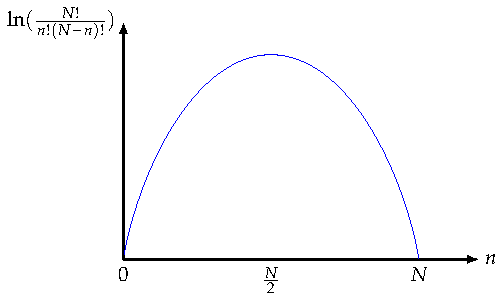
\includegraphics[]{Images/fig-TLSstatecounting.pdf}
    
    \caption{Plot of (continuum approximation) $\ln\frac{N!}{n!(N-n)!}$ as a function of number of spin-up spins $n$. We see the maximum at $n = N/2$ (zero magnetization).}
    \label{fig-TLSstatecounting}
\end{figure}

so indeed the state with $n = N/2$ spins up (and $n = N/2$ spins down) - the state with total magnetization $m = 0$ is the most probable state. It is also valuable to ask what fraction of the total number of states is the most likely distribution. This is simply obtained by taking the number of states with $n = N/2$ and dividing by the total $2^n$:
\begin{equation}
    \frac{N!}{(N/2)!(N/2)!} \frac{1}{2^{n}}
\end{equation}
We find that (using Stirling's formula that):
\begin{equation}
    \ln( \frac{N!}{(N/2)!(N/2)!} \frac{1}{2^{N}}) = 0 + \frac{\ln N}{N}
\end{equation}
so in the $N \to \infty$ limit, $\frac{N!}{(N/2)!(N/2)!} \frac{1}{2^{N}} \approx 1$ to leading order, so the proportion of the most likely distribution to total states of the system is one (with corrections given by the successive terms).
\section{Free Energy, Ideal Gas, and the Grand Canonical Ensemble}

\subsection{Thermodynamic Interpretation, Energy, and Free Energy}
Last time, we looked at the canonical ensemble. We derived the most probable distribution:
\begin{equation}
    \rho_a = \frac{e^{-\beta E_a}}{\sum_a e^{-\beta E_a}}
\end{equation}
and found the partition function:
\begin{equation}
    Z = \sum_a e^{-\beta E_a}.
\end{equation}
We argue that this already has a nice thermodynamic interpretation. This comes about if we look at the logarithm of the partition function:
\begin{equation}
    F = -\frac{1}{\beta}\ln Z = -\frac{1}{\beta}\ln \sum_a e^{-\beta E_a}
\end{equation}
Note that if there was only one energy level, then this would immediately just be the energy - in general the energy we calculate as the expectation value:
\begin{equation}
    U = \frac{\sum_a E_a e^{-\beta E_a}}{\sum_a e^{-\beta E_a}}
\end{equation}
How does $F$ relate to $U$? Let us write:
\begin{equation}
    F = U + \left(-\frac{1}{\beta}\ln \sum_a e^{-\beta E_a} - \frac{\sum_a E_a e^{-\beta E_a}}{\sum_a e^{-\beta E_a}}\right)
\end{equation}
Let us call $e^{-\beta E_a} = Z \rho_a$ and write $E_a = -\frac{1}{\beta}\ln Z - \frac{1}{\beta}\ln \rho_a$. Then, rewriting the above expression, we find:
\begin{equation}
    F = U - \frac{1}{\beta}\sum_a \rho_a \ln \rho_a.
\end{equation}
The second term should be familiar to anyone with an information theory background - $S_{VN} = \sum_a \rho_a \ln \rho_a$ is known as the von Neumann entropy. It is the entropy of the distribution - a measure of how little we know about the system when we have the distribution $\rho_a$. It is minimized if one of the $\rho$s is one and the others are zero, as the entropy is zero (then we know exactly what the system is). It is maximized if all of the $\rho$s are constant (because then we know nothing about the system). If we are willing to accept that the von Neumann entropy is equal to the thermal entropy up to a constant:
\begin{equation}
    S = k_B S_{VN}
\end{equation}
where $k_B$ is Boltzmann's constant. Then, we obtain:
\begin{equation}
    F = U - \frac{1}{\beta}\frac{S}{k_B}
\end{equation}
which closely resembles:
\begin{equation}
    F = U - TS. 
\end{equation}
where $T$ is the temperature (if we interpret $\beta = \frac{1}{k_B T}$). This is the familiar thermodynamic expression for the Helmholtz free energy.

This is not the historical order in which things are done - historically the microcanonical viewpoint (due to Boltzmann) came first, but this requires the system to be thermodynamic.

\subsection{Example - System of weakly interacting non-relativistic particles}
Let us assume we have a collection of $N$ weakly interacting non-relativistic particles of mass $m$, which obey the laws of classical mechanics. A state of such a system will just be the specifications of the positions and velocity (or momenta) of all the particles (mathematically, this is because Newton's second law is a second-order ODE so we require two boundary conditions to specify the state). We can write the state as a collection of these values $\set{\v{q}_1, \v{p}_1, \ldots, \v{q}_n, \v{p}_n}$ The energy is then given by the Hamiltonian:
\begin{equation}
    H = \sum_k \frac{\v{p}_k^2}{2m}
\end{equation}
Note we assume that the masses of the particles are the same and all attributes of the particles (other than position or momentum) are identical - note that in the context of classical mechanics this does not make the particles indistinguishable - we can keep track of them. This is in contrast to quantum statistical mechanics, where particles are truly indistinguishable and are either fermions or bosons.

We can construct the partition function for this system:
\begin{equation}
    Z = \int d\v{q}_1 d\v{p}_1 \ldots d\v{q}_n d\v{p}_n e^{-\beta H}
\end{equation}
this looks reasonable, but there are a couple things wrong with this. One problem - $Z$ has dimensions; this is problematic if we want to take functions of it (e.g. logarithms to get the free energy). To deal with this problem, we just divide it by a number that gets rid of the dimensions:
\begin{equation}
    Z = \frac{1}{(2\pi \hbar)^{3N}}\int d\v{q}_1 d\v{p}_1 \ldots d\v{q}_n d\v{p}_n e^{-\beta H}
\end{equation}
$\hbar$ we pretty much pulled out of a hat here, but we require something with the dimensions of angular momentum to place there. Let's now do the integral. Let's assume that our particles move in infinite 3-D Euclidean space; we can then write $\int d\v{q}_i = V$ (the volume) as $H$ does not depend on the positions. Further, all momentum integrals are equivalent, so let us write it as the product of momentum integrals:
\begin{equation}
    Z = \frac{V^N}{(2\pi \hbar)^{3N}}\left(\int dp e^{-\frac{\beta}{2m}\v{p}^2}\right)^{3N}
\end{equation}
We go into polar coordinates to solve this Gaussian integral:
\begin{equation}
    \left(\int dp\right)^{3N} \to \left(\int d^2p\right)^{\frac{3N}{2}} \to \left(\int \frac{d\phi pdp}{2}\right)^{\frac{3N}{2}}
\end{equation}
which yields:
\begin{equation}
    Z = \frac{V^N}{(2\pi \hbar)^{3N}} \left(\frac{2\pi m}{\beta}\right)^{\frac{3N}{2}} = V^N\left(\frac{mk_B T}{2\pi \hbar^2}\right)^{\frac{3N}{2}}
\end{equation}
The Helmholtz free energy is then:
\begin{equation}
    F[T, V, N] = -k_B T N\ln \left[V\left(\frac{mk_B T}{2\pi \hbar^2}\right)^{3/2}\right]
\end{equation}
This system should be truly thermodynamic (as we can take the system to be large), so this should work - we will see in a moment that unfortunately, it does not!

Recall thermodynamic differential relation:
\begin{equation}
    dF = -S dT + \mu dN - P dV
\end{equation}
So the entropy is:
\begin{equation}
    S = \left.-\dpd{F}{T}\right|_{N, V}
\end{equation}
the chemical potential is:
\begin{equation}
    \mu = \left.\dpd{F}{N}\right|_{T, V}
\end{equation}
and the pressure is:
\begin{equation}
    P = \left.-\dpd{F}{V}\right|_{T, N}
\end{equation}
so we can go to town and calculate some quantities. For example
the pressure we can calculate to be:
\begin{equation}
    P = \frac{N k_B T}{V}
\end{equation}
which is the ideal gas law! Big success (the other quantities will not be as successful...)! The chemical potential we can calculate to be:
\begin{equation}
    \mu = -k_B T\ln\left(V\left(\frac{mk_B T}{2\pi \hbar^2}\right)^{3/2}\right)
\end{equation}
The entropy we calculate to be:
\begin{equation}
    S = \frac{3}{2}k_B N + k_B N\ln\left(V\left(\frac{m k_B T}{2\pi \hbar^2}\right)^{3/2}\right)
\end{equation}
We can calculate the energy to be:
\begin{equation}
    U = F + TS = \frac{3}{2}N k_B T
\end{equation}
which is again a beautiful formula (and the correct result). However, we should talk about why the formulas for $\mu, S$ are wrong. They do not have the correct extensivity properties. Concretely, if one considers two identical volumes of ideal gas separated by a partition, removing and re-inserting the partition should be reversible. However, a calculation of the entropy change shows that removing the partition leads to an increase in entropy of $2k_B N \ln 2$; contradiction. So we're a failure. But we're also clever, and can try to fix it. We introduce a factor of $\frac{1}{N!}$ into the partition function. This introduces a factor of $\frac{1}{N}$ into the logarithm in the free energy expression, which ends up correcting things. This was originally a fudge factor fix, but it turns out to be quite deep - namely, we have overcounted the states in the system somehow, and the $\frac{1}{N!}$ corrects for this. This hints to classical mechanics being problematic (quantum statistics fixes this with indistinguishability). 

But let's try taking $Z \to \frac{1}{N!}Z$ (we are exploring what is known as Maxwell-Boltzmann statistics). Then with Stirling's formula:
\begin{equation}
    \ln N! \approx N\ln N - N = \ln \left(\frac{N}{e}\right)^N
\end{equation}
Then the free energy becomes:
\begin{equation}
    F[T, N, V] = -k_B T\ln\left[\frac{eV}{N}\left(\frac{mk_B T}{2\pi \hbar^2}\right)^{3/2}\right]
\end{equation}
and now we see that $F$ has the correct scaling properties so things have been fixed. If we now recalculate quantities, $P, U$ stay the same (as beautiful as they were):
\begin{equation}
    PV = Nk_B T
\end{equation}
\begin{equation}
    \frac{U}{N} = \frac{3}{2}k_B T
\end{equation}

And now the entropy is fixed up as well:
\begin{equation}
    S = \frac{3}{2}k_B N + k_B N\ln\left(\frac{eV}{N}\left(\frac{mk_B T}{2\pi\hbar^2}\right)^{3/2}\right)
\end{equation}
and this is known as the \emph{Sackur-Tetrode equation}.

Before we go on - there are other ensembles we could have used, e.g. the grand canonical ensembles where the subsystems are allowed to exchange particles as well as energy. We need this as this one is the easier one to use when we consider quantum statistics. So in a way, Maxwell-Boltzmann statistics assumes the distribution is completely symmetric in the particles, but it is blind to how the wavefunction changes - if we take the distribution to be $\rho = \psi^\dag \psi$, it assumes that each permutation comes out to be symmetric. But is not actually completely correct as in QM we impose the proper statistics on the wavefunctions, rather than the density.

\subsection{Grand Canonical Ensemble}
The logic follows exactly the same as the Canonical ensemble, with the only difference that we allow for the particle number to change. Suppose a system has $N_a$ particles in state $a$, and energy $E_a$. We define $n_a$ to be the number of systems in the ensemble in state $a$. We have some constraints:
\begin{equation}
    \sum_a n_a = \mathcal{N}
\end{equation}
\begin{equation}
    \sum_a n_a E_a = \mathcal{E} = \mathcal{N}U
\end{equation} 
\begin{equation}
    \sum_a n_a N_a = \mathcal{N}N
\end{equation}
in the above, $U$ is the average energy and $N$ is the average number of particles. This differs from what we had before by one equation. We want to find the most probable distribution; for this the mathematics is exactly the same, just with one more Lagrange multiplier. We maximize:
\begin{equation}
    \ln \frac{\mathcal{N}!}{\prod_a n_a !} + \beta(U\mathcal{N} - \sum_a n_a E_a) + \alpha\left(N\mathcal{N} - \sum_a n_a N_a\right) + \gamma\left(\mathcal{N} - \sum_a n_a\right)
\end{equation}
The argument is basically identical to what we did to calculate $\rho_a$ for the canonical ensemble. We solve the first and last equations for $\rho_a$ and leave the other two unsolved (they will be thermodynamic quantities we can interpret). After the dust settles, we end up with:
\begin{equation}
    \rho_a = \frac{e^{-\beta E_a - \alpha N_a}}{\sum_a e^{-\beta E_a - \alpha N_a}}
\end{equation}
Our grand canonical partition function is:
\begin{equation}
    \mathcal{Z} = \sum_a e^{-\beta E_a - \alpha N_a}
\end{equation}
If we identify:
\begin{equation}
    \Phi = -k_B T \ln \mathcal{Z}
\end{equation}
with the grand canonical free energy, and go through a similar procedure of identifying the Von Neumann entropy with the thermodynamic entropy (and an identification to relate $\alpha$ with the chemical potential), we obtain:
\begin{equation}
    \beta = -\frac{1}{k_B T}, \quad \alpha = -\frac{\mu}{k_B T}.
\end{equation}
The grand canonical free energy now no longer depends on the number of particles, but on the chemical potential. It is however related to the Helmholtz free energy via a Legendre transform:
\begin{equation}
    \Phi[T, \mu, V] = F - \mu \mathcal{N}
\end{equation}
If we did things correctly, working with the grand canonical free energy vs. the Helmholtz free energy should yield the same answers. If we recall the canonical partition function for the weakly interacting gas, we had a dependence on the particle number $N$ (note - NOT the average number of particles in the systems of the ensemble, but here really the number of particles in the ideal gas. Sorry for the overload of notation). We can sum over $N$ to get the grand canonical partition function. We can then go through and see if we obtain the same results (and we will). We had:
\begin{equation}
    Z[T, N, V] = \frac{1}{N!}V^N\left(\frac{mk_B T}{2\pi \hbar^2}\right)^{\frac{3N}{2}}
\end{equation}
note the inclusion of the $\frac{1}{N!}$ factor so things end up correct. The grand canonical partition function is then:
\begin{equation}
    \mathcal{Z}[T, \mu, V] = \sum_N e^{\frac{\mu}{k_B T}N}Z[T, N, V]
\end{equation}
this is an easy sum because its just $\sum_N \frac{1}{N!}x^N$; hopefully this is familiar as just an exponential:
\begin{equation}
    \mathcal{Z}[T, \mu, V] = e^{V\left(\frac{mk_B T}{2\pi \hbar^2}\right)^{3/2}e^{\frac{\mu}{k_B T}}}
\end{equation}
so our prediction for the grand canonical free energy is:
\begin{equation}
    \Phi = -k_B T \ln \mathcal{Z} = -k_B TV\left(\frac{mk_B T}{2\pi \hbar^2}\right)^{3/2}e^{\frac{\mu}{k_B T}}
\end{equation}
and we can go through the song and dance to obtain the quantities that we solved for using the canonical ensemble.

\end{document}